\chapter{考察}
\label{ch:discussion}
\ref{ch:discussion}章ではミリ波分光計を用いて得られた\ref{ch:results}章での結果と、ミリ波分光計以外の外部からのデータの比較とを行う。
\ref{sec:comparison_sofie}節では、ノルウェー・トロムソにおける解析結果(\ref{sec:results_tromsoe}節)に対し、SOFIE(Solar Occultation for Ice Experiment。詳細は付録~\ref{app:sofie})衛星によって観測された\ce{NO}密度の高度プロファイルデータを用いて比較を行う。
\ref{sec:comparison_eep}節では、観測された\ce{NO}柱密度の変動に対するEPPの影響を調べるため、POES/MetOp衛星で観測された降り込み電子や地磁気擾乱指数との比較を行う。


\section{SOFIEの観測データから導出されたNO柱密度との比較}
\label{sec:comparison_sofie}
まずは、ミリ波分光計を用いた\ce{NO}の観測データの妥当性を検証するため、SOFIEによって観測された\ce{NO}の高度プロファイルデータと比較する。
使用したSOFIEのデータは、トロムソで\ce{NO}柱密度を導出した期間と同じ期間にトロムソ付近の緯度(およそ$65 - 80$\textdegree Nの範囲)で観測された高度ごとの\ce{NO}密度である。
なお、昭和基地においては、ミリ波分光計のデータ解析を行った期間のSOFIEによる観測データが\today 時点で公開されていないため、比較を行うことはできなかった。
% 仮綴じでは today = 2024-01-26となっている。
したがって、\ref{sec:comparison_sofie}節ではトロムソでの比較結果についてのみ述べる。\par

図~\ref{fig:sofie_mmcd}に、SOFIEによって得られた\ce{NO}密度の高度プロファイル(a)と、ミリ波分光計によって得られた\ce{NO}柱密度の時間変化((b)の白抜き丸プロット)を示す。
\begin{figure}[htbp]
    \centering
    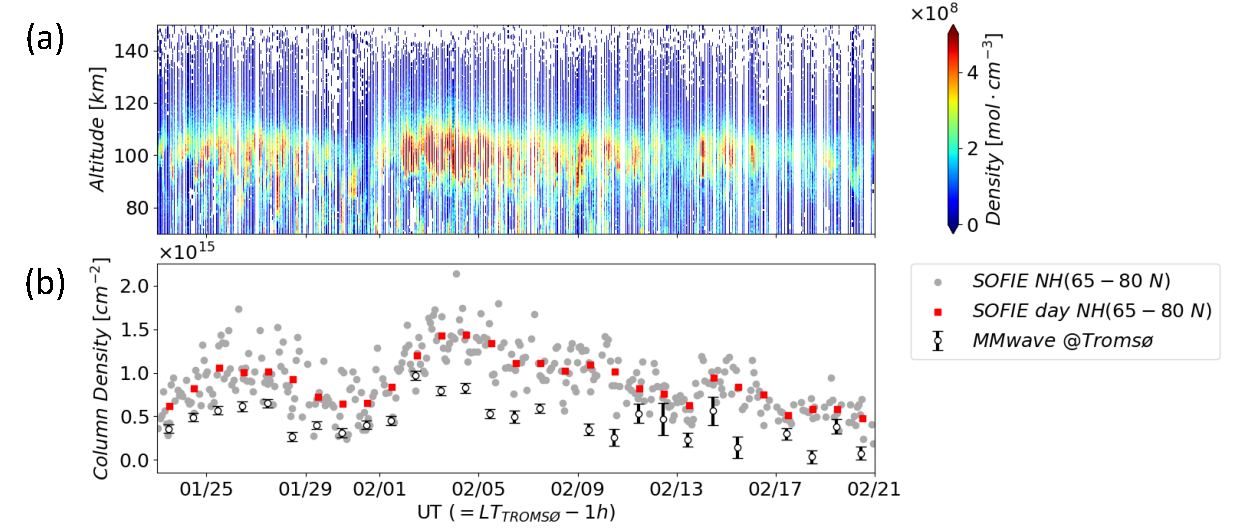
\includegraphics[width=\linewidth]{master_thesis_contents/master_thesis_fig/sofie_mmcd.pdf}
    \caption{(a)SOFIEの\ce{NO}密度の高度プロファイルデータおよび(b)ミリ波分光計を用いて導出したトロムソの柱密度とSOFIEの\ce{NO}密度の高度プロファイルデータから導出した柱密度の比較(エラーバー付きのプロットがミリ波データから導出した柱密度、グレーの丸形プロットがSOFIEの\ce{NO}密度の高度プロファイルデータから導出した柱密度、赤色の四角プロットが1日平均したSOFIEの柱密度)}
    \label{fig:sofie_mmcd}
\end{figure}
ミリ波分光計によって柱密度の増加が確認された2つの期間(2019年1月23日〜2019年1月27日と2019年2月1日〜2019年2月4日)では、SOFIEの高度プロファイルデータでも高度$100\ \mathrm{km}$付近において\ce{NO}の密度の増加が確認できた。\par

また、ミリ波分光計を用いて導出した柱密度とSOFIEのデータを直接比較をするため、SOFIEの\ce{NO}密度の高度プロファイルを高度方向に足し合わせることで、柱密度を導出した(図~\ref{fig:sofie_mmcd}(b)のグレーの丸形プロット)。
これをさらに1日平均した値が図~\ref{fig:sofie_mmcd}(b)の赤い四角プロットである。
これらを比較した結果、ミリ波分光計による柱密度の時間変動の傾向は、SOFIEから導出した柱密度の傾向とよく一致していることが分かった。
しかし、全体的にSOFIEから導出した柱密度の方が、ミリ波分光計による柱密度と比べて値が大きいことも分かった。\par

ここで、図~\ref{fig:sofie_mmcd}(b)を見ると、ミリ波分光計を用いて導出した柱密度のほうが常に一定の割合で低く見積もっているように見えるため、SOFIEから導出した柱密度とミリ波分光計による柱密度には定常倍のオフセットがあると仮定して二値の比較を行った。
\begin{figure}[htbp]
    \centering
    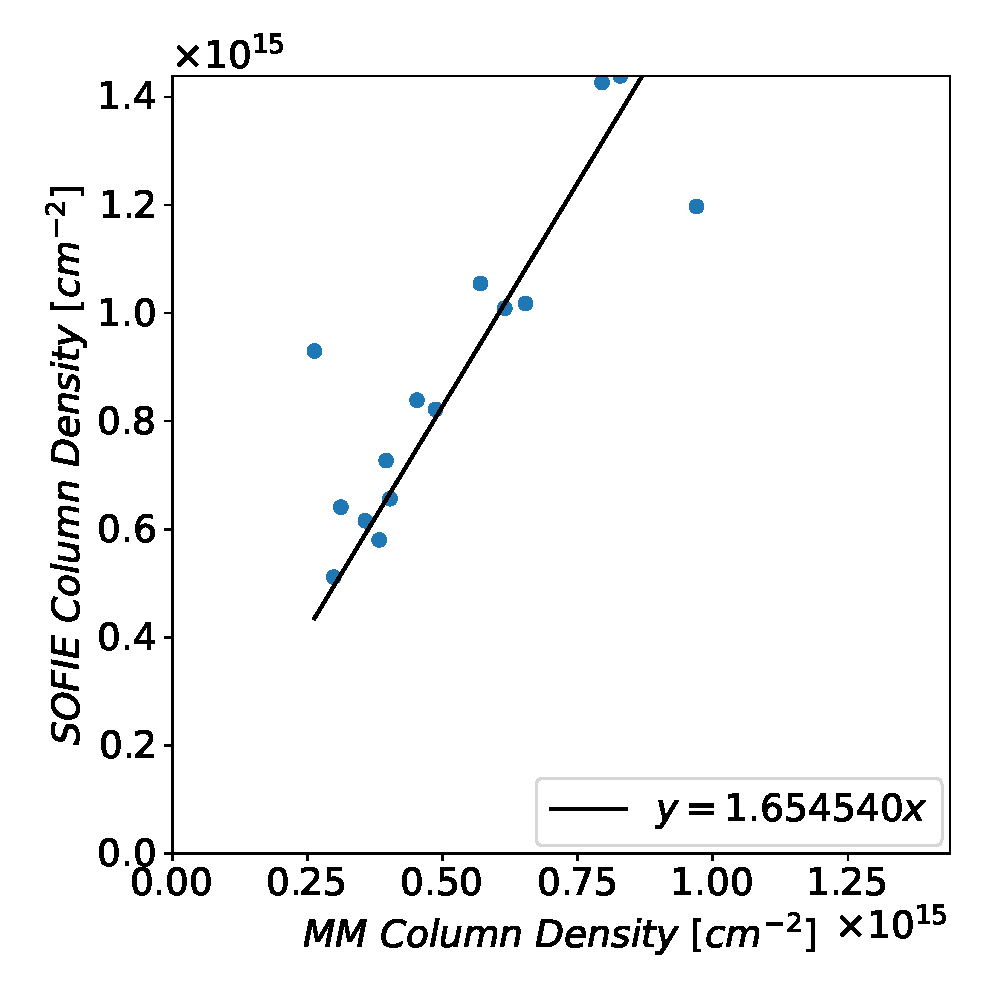
\includegraphics[scale=0.5]{master_thesis_contents/master_thesis_fig/sofie_mmcd_sofiecd_corr.pdf}
    \caption{ミリ波分光計から求めた柱密度(横軸)とSOFIEデータから求めた柱密度の1日平均値(縦軸)との散布図(青色のプロット。黒線は一次近似による直線を示し、右下はその式を表している)}
    \label{fig:sofie_mmcd_sofiecd_corr}
\end{figure}
ミリ波分光計から求めた柱密度と、SOFIEデータから求めた柱密度の1日平均値について、散布図を作成した結果を図~\ref{fig:sofie_mmcd_sofiecd_corr}に示す。
ただし、ミリ波のデータでスクリーニングされた期間(2019年2月5日〜2019年2月16日)と、検知限界($2\times 10^{14}\ \mathrm{cm^{-2}}$)を下回るデータは含めていない。
ここで、近似直線は、SOFIEから導出した柱密度とミリ波分光計による柱密度には定常倍のオフセットがあるとする仮定より、切片を0に固定している(図~\ref{fig:sofie_mmcd_sofiecd_corr}の黒線。近似直線の式は図の右下に示す)。
この図より、SOFIEによる\ce{NO}柱密度はミリ波分光計による柱密度のおよそ1.65倍の大きさであることが分かった。\par

この原因のひとつとして考えられるのは、ミリ波分光計で柱密度を導出する際に仮定した大気温度(\ref{sec:derive_columndensity}節の式\eqref{eq:derive_columndensity}の第2項$T_{\mathrm{atm}}$)の値が妥当ではない可能性である。
そこで、NRLMSIS 2.0\footnote{\url{https://ccmc.gsfc.nasa.gov/models/NRLMSIS~00/}}を用いて、大気温度の妥当な値を調べた。
NRLMSIS 2.0とは地上から大気圏外までの経験的な大気モデルで、温度・8種類の数密度・質量密度の平均的な観測挙動を表すものであり、大気温度の高度プロファイルを調べることができる。\par

これを用いて、2019年1月25日と2月2日(ミリ波分光計を用いて導出した\ce{NO}の柱密度の時間変動のピーク)における高度$100\ \mathrm{km}$付近(SOFIEの\ce{NO}の密度の高度プロファイルデータにおける、ピークがある高度)の大気温度を調べたところ、およそ$180-250\ \mathrm{K}$の範囲であった。
仮に$250\ \mathrm{K}$に仮定し直すと、ミリ波分光計を用いて導出した\ce{NO}の柱密度は1.25倍される。
しかし、これだけではSOFIEで導出した\ce{NO}の柱密度との値の差をすべて説明することはできない。
大気温度を高度に依存せず一様と仮定していることもオフセットの原因として考えられるため、大気温度を高度ごとに設定することも考慮に入れる必要があると考えている。
これは今後の課題である。\par

繰り返しになるが、解析期間内において北半球の高緯度領域(およそ$65 - 80$\textdegree Nの範囲)を全体的に観測を行うSOFIEと、トロムソで一定点観測を行うミリ波分光計では、観測の対象領域に違いがあるため、全球的な傾向とトロムソでの局地的な傾向が異なる可能性もある。
これに関しては、Box Trajectory手法(放出される大気中の粒子をBoxに見立てて、そのBoxの中でどのような化学反応が起きるか計算をし、そのBoxがどのように動いていくのかの解析を行う)を用いたモデル計算の結果とミリ波分光計による観測結果と比較すれば、それぞれで導出したトロムソでの局地的傾向を比較することができるので、解決できる可能性が考えられる。


\section{高エネルギー電子の降り込みとの比較}
\label{sec:comparison_eep}
次に、ミリ波分光計の観測から見出された\ce{NO}柱密度変動に対するEPPの影響を調べるため、高エネルギー電子の降り込みの指標となるデータとの比較を行った。
比較対象として以下の3種類のデータを用い、各節に分けて比較結果を述べる。
\begin{itemize}
    \item Dst指数(\ref{ssec:comparison_dst}節)
    \item POES/MetOp衛星で観測された電子フラックスデータ(\ref{ssec:comparison_poes}節)
    \item NASAが提供しているOMNI Data Set(\ref{ssec:comparison_omni}節)
\end{itemize} \par
Dst指数、POES/MetOp、OMNI Data Setの詳細は、それぞれ付録~\ref{app:dst}、付録~\ref{app:poes}、付録~\ref{app:omni}にて紹介している。


\subsection{Dst指数との比較}
\label{ssec:comparison_dst}
まずは、Dst指数との比較を行った。
Dst指数とは、地磁気擾乱の大きさを表す指数であり、地磁気擾乱が起きた際にその値が負方向に変化する。
これは、地球を取り巻く環状の電流(Ring Current)が、どの程度地球磁場を打ち消すかを数値的に表したものである(詳細は付録~\ref{app:dst})。
Dst指数のデータは、地磁気世界資料センター京都(WDC for Geomagnetism, Kyoto)\footnote{\url{https://wdc.kugi.kyoto-u.ac.jp/wdc/Sec3.html}}より調べた。\par
Dst指数とトロムソにおける\ce{NO}柱密度との比較結果を図~\ref{fig:dst_mmcd_tromsoe}、昭和基地における比較結果を図~\ref{fig:dst_mmcd_syowa}に示す。
\begin{figure}[htbp]
    \centering
    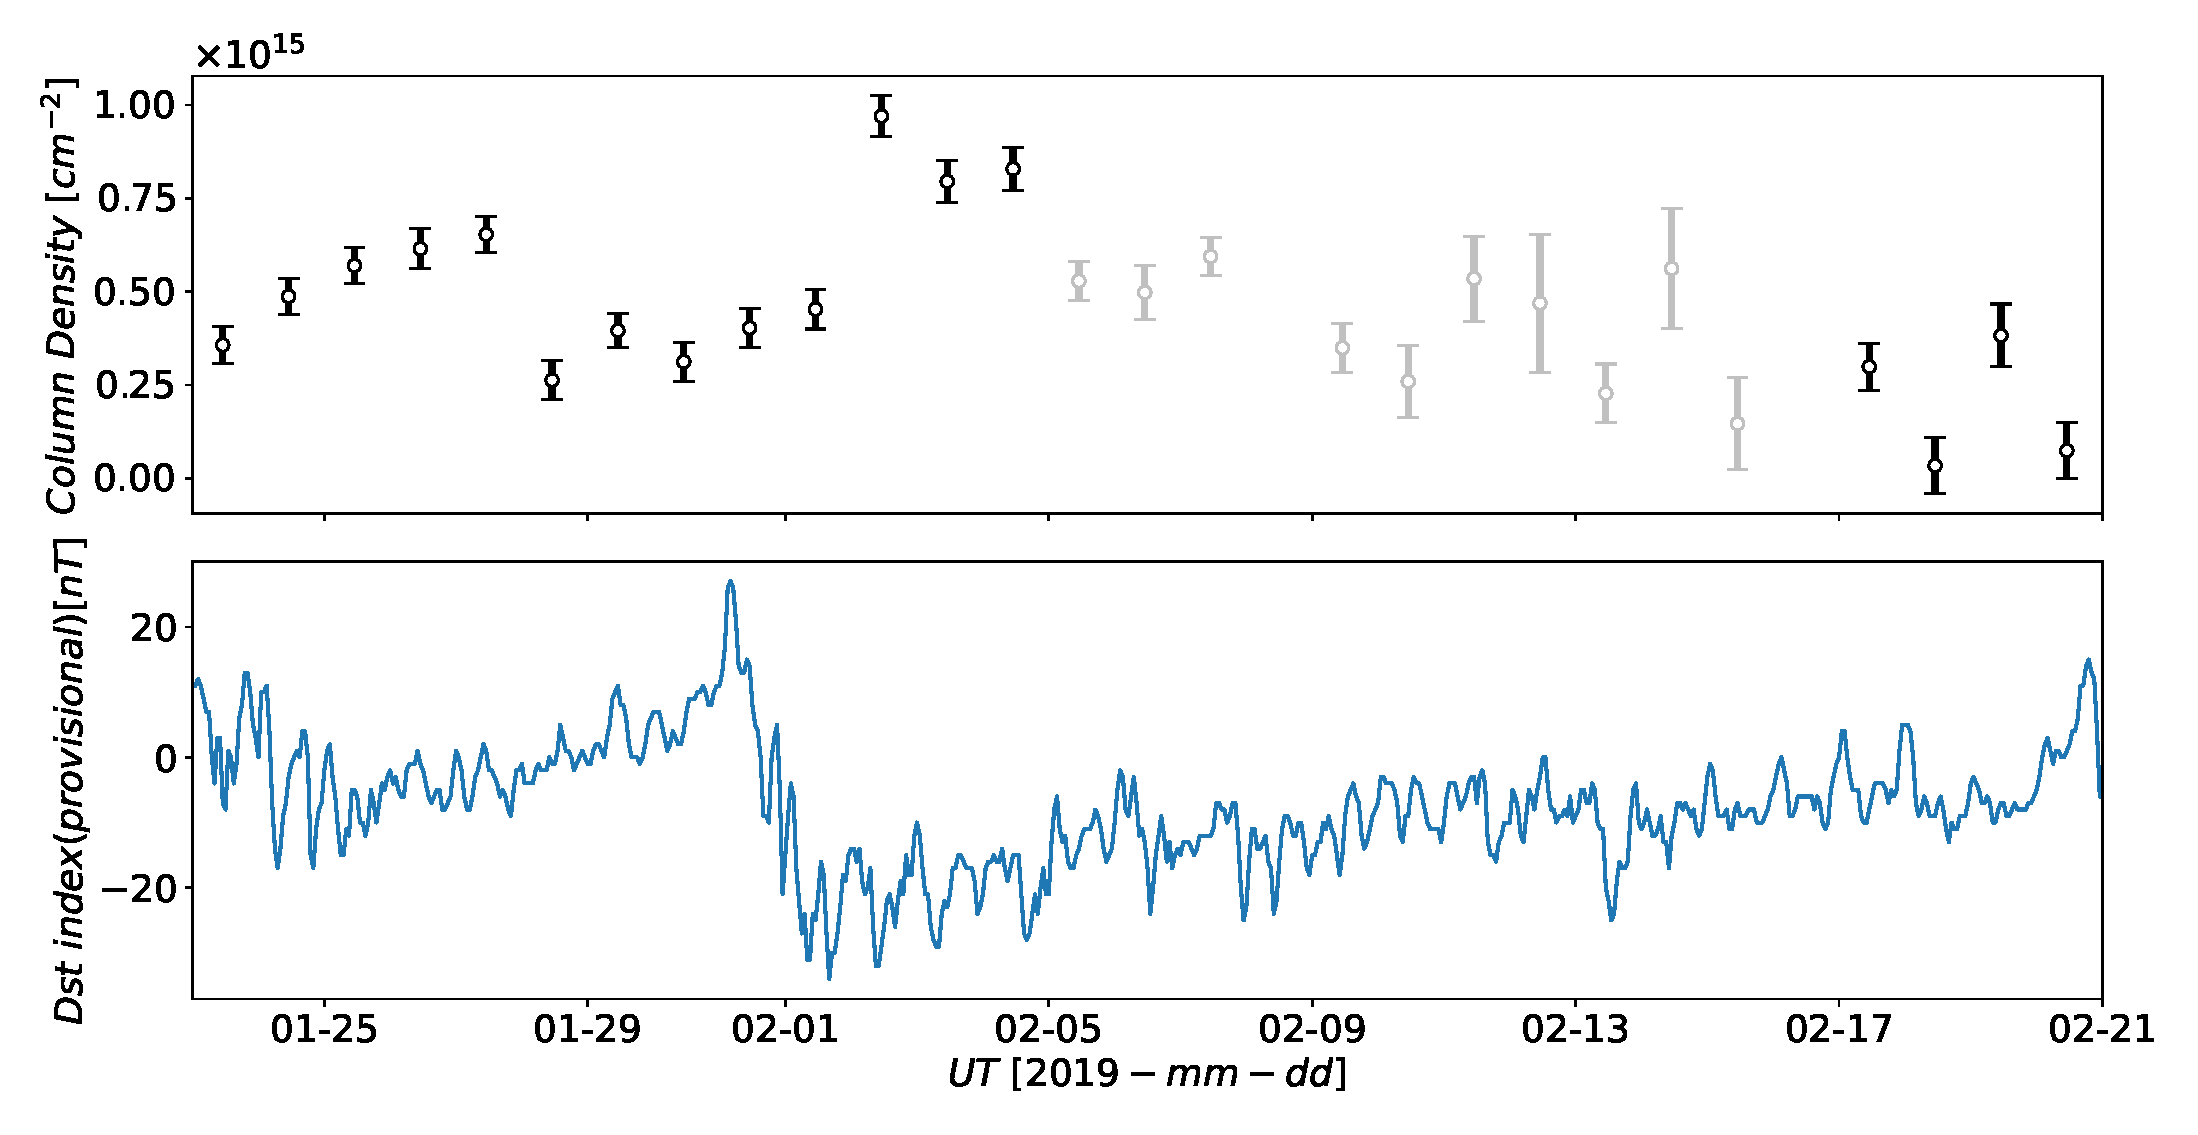
\includegraphics[width=\linewidth]{master_thesis_contents/master_thesis_fig/dst_tromsoe_mmcd.pdf}
    \caption{トロムソにおける柱密度(1段目。図~\ref{fig:column_density_spectr6_syowa}と同様)とDst指数 暫定値(2段目)との比較}
    \label{fig:dst_mmcd_tromsoe}
\end{figure}
\begin{figure}[htbp]
    \centering
    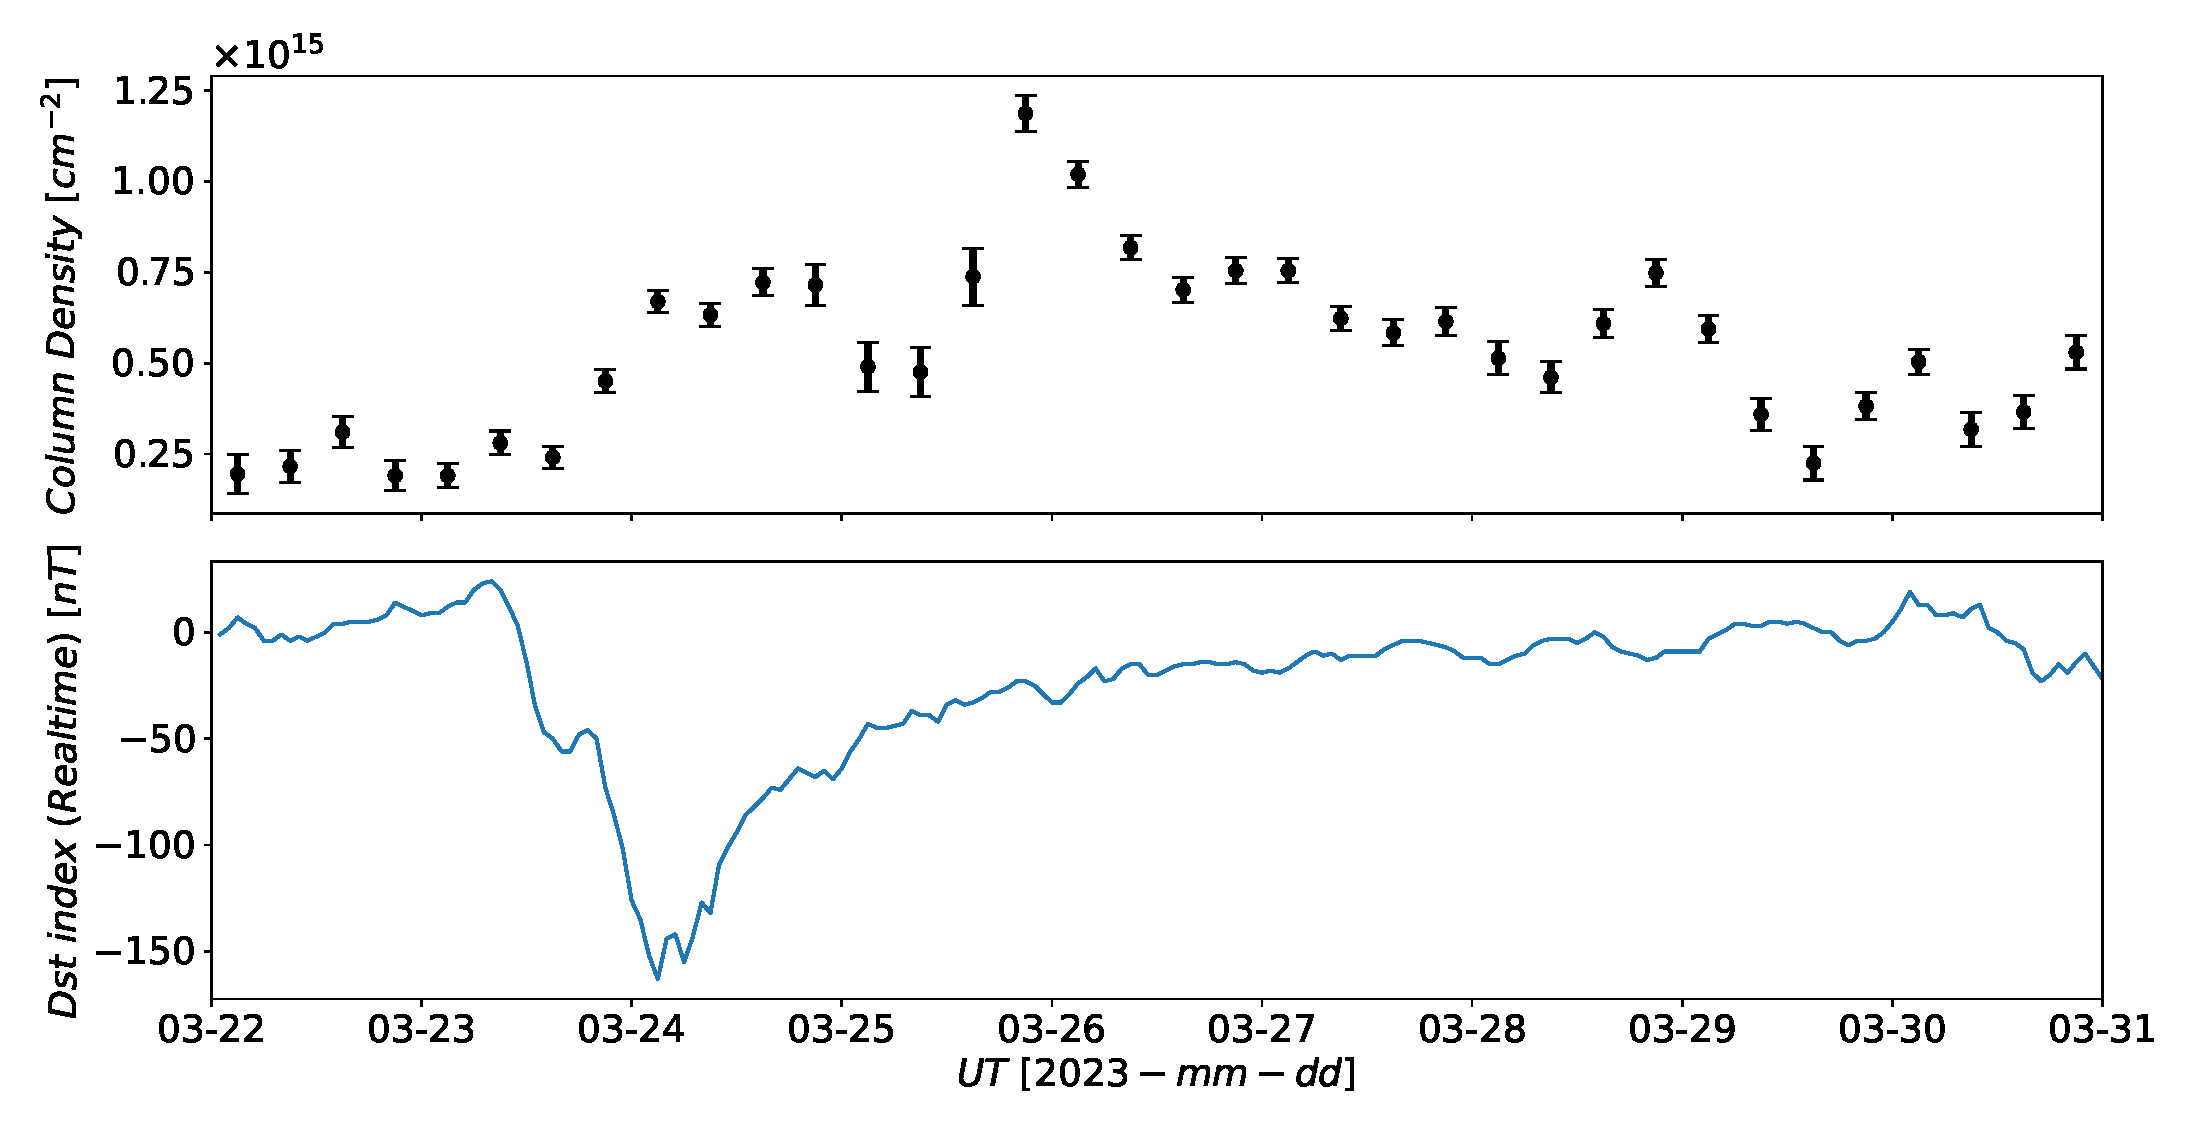
\includegraphics[width=\linewidth]{master_thesis_contents/master_thesis_fig/column_density_spectr6_dst_syowa.pdf}
    \caption{昭和基地における柱密度(1段目。図~\ref{fig:column_density_spectr6_syowa}と同様)とDst指数 速報値(2段目)との比較}
    \label{fig:dst_mmcd_syowa}
\end{figure}
どちらの比較においても、\ce{NO}の柱密度の増加が確認できた期間に対応して、Dst指数の急激な減少がみられた。
とくに、トロムソにおいては急激な\ce{NO}の柱密度の増加があった2019年2月1日〜2019年2月4日、昭和基地においては2023年3月24日の未明前後における\ce{NO}の柱密度の増加によく対応している。
また、比較的小規模ではあるが、トロムソにおいては2019年1月23日〜2019年1月27日においても、Dst指数の減少が確認された。\par

この結果より地磁気擾乱によって加速されて極域に降り込んだ電子により、\ce{NO}が増加した可能性が考えられる。
しかし、それ以外で\ce{NO}の柱密度の増加が確認できた期間(昭和基地における2023年3月23日21時〜2023年3月24日3時)については、Dst指数の減少は確認できなかった。
これは、地磁気擾乱による原因以外で\ce{NO}の増加に寄与するものがあると考えられる(これについては以下の\ref{ssec:comparison_poes}節・\ref{ssec:comparison_omni}節で述べる)。


\subsection{POES/MetOp衛星の電子フラックスデータとの比較}
\label{ssec:comparison_poes}
次に、電子の降り込みが起きているとき、どのようなエネルギーレンジの電子が影響しているかを調べるため、POES/MetOp衛星の電子フラックスデータとの比較を行った。
まず、ミリ波分光計の観測場所周辺に降り込む電子のフラックスのみを調べるため、用いるデータについては事前に絞り込みを行った(詳細は付録~\ref{app:poes})。
トロムソと昭和基地における比較結果をそれぞれ図~\ref{fig:poes_mmcd_tromsoe}、図~\ref{fig:poes_mmcd_syowa}に示す。
なお、電子フラックスデータは、電子がもつエネルギーについて4つの範囲($>40\ \mathrm{keV}$, $>130\ \mathrm{keV}$, $>287\ \mathrm{keV}$, $>612\ \mathrm{keV}$)に分け、それぞれ別のグラフで示してある。
\begin{figure}[htbp]
    \centering
    \begin{minipage}{\linewidth}
        \centering
        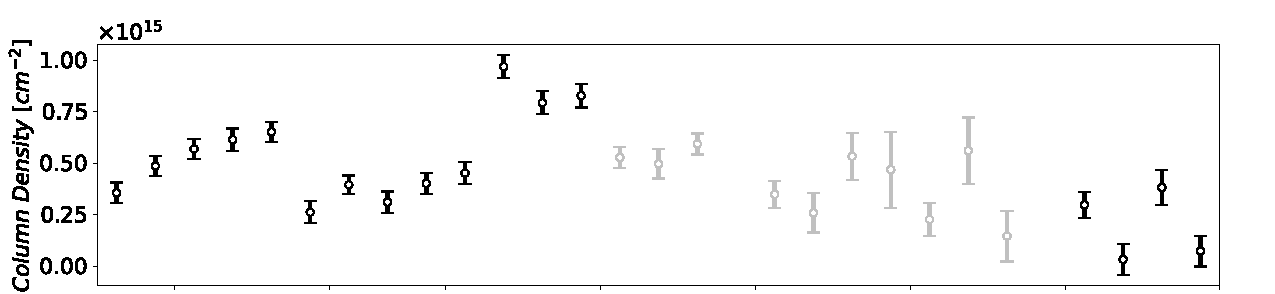
\includegraphics[width=\linewidth]{master_thesis_contents/master_thesis_fig/avg_ColumnDensity_tromsoe_trim.pdf}
    \end{minipage}
    \begin{minipage}{\linewidth}
        \centering
        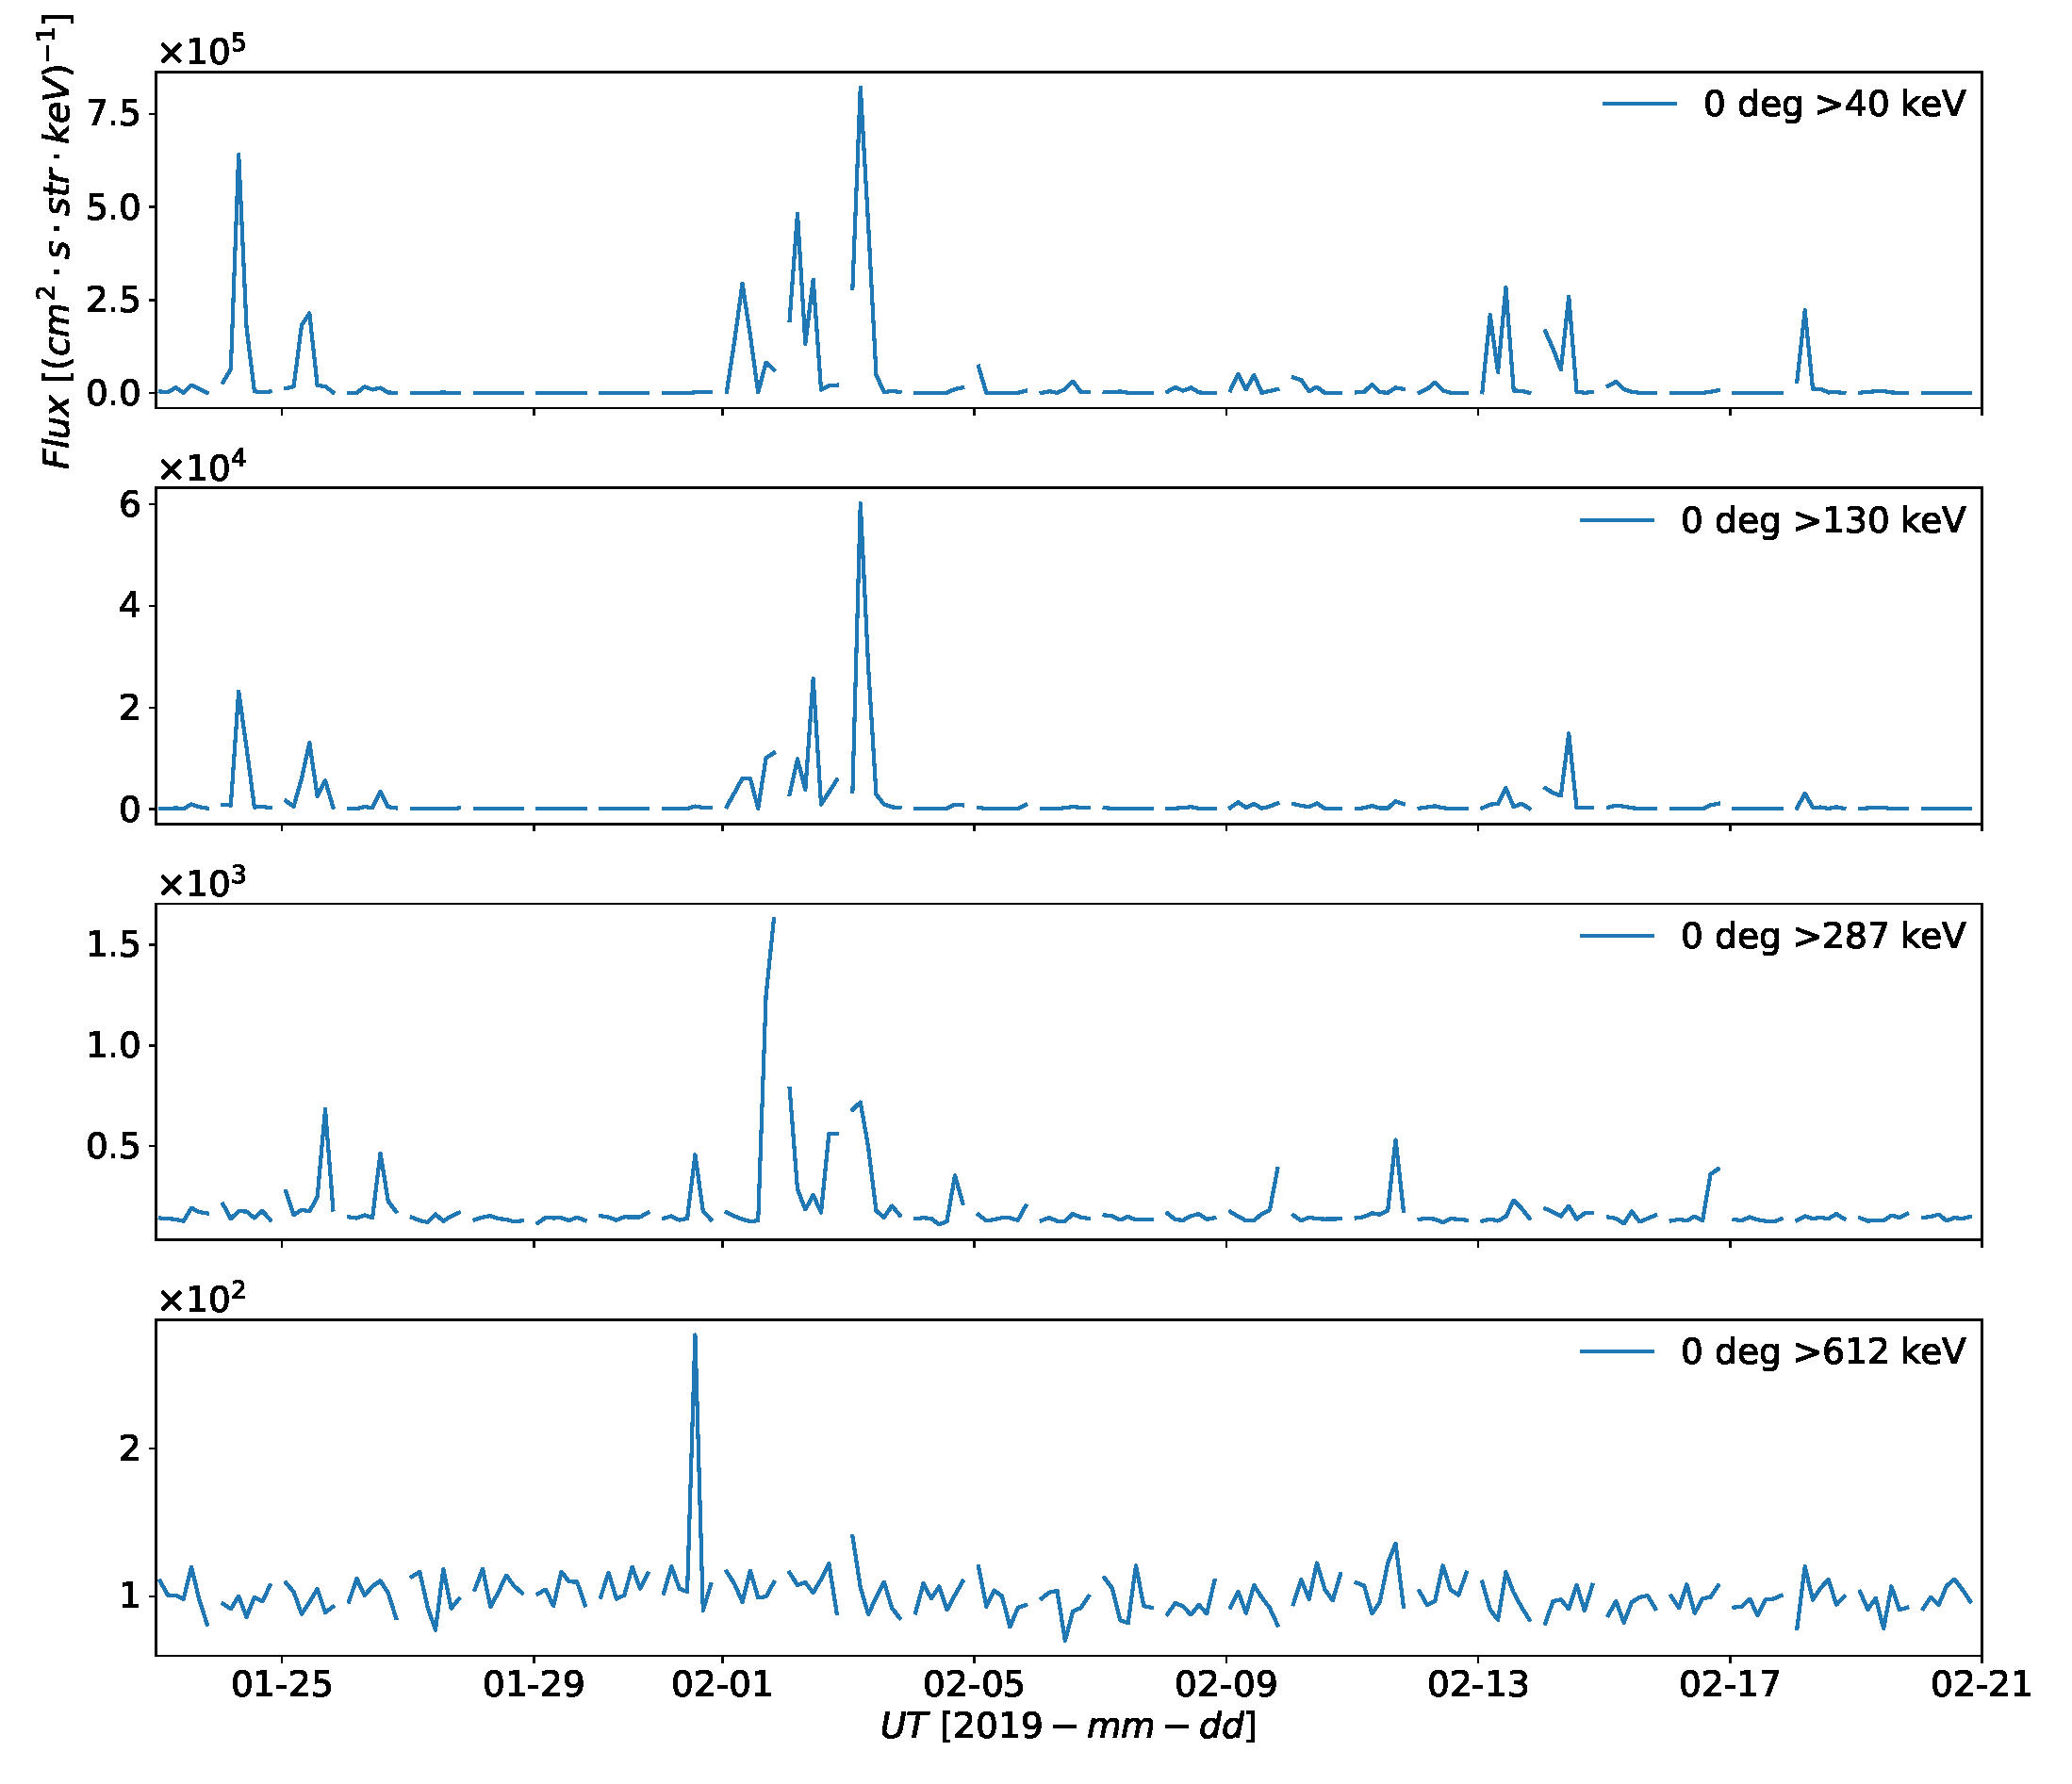
\includegraphics[width=\linewidth]{master_thesis_contents/master_thesis_fig/poes_tromsoe_0deg.pdf}
    \end{minipage}
    \caption{トロムソにおける柱密度(1段目。図~\ref{fig:avg_ColumnDensity_tromsoe}と同様)と電子フラックスデータ(2-5段目)との比較}
    \label{fig:poes_mmcd_tromsoe}
\end{figure}
\begin{figure}[htbp]
    \centering
    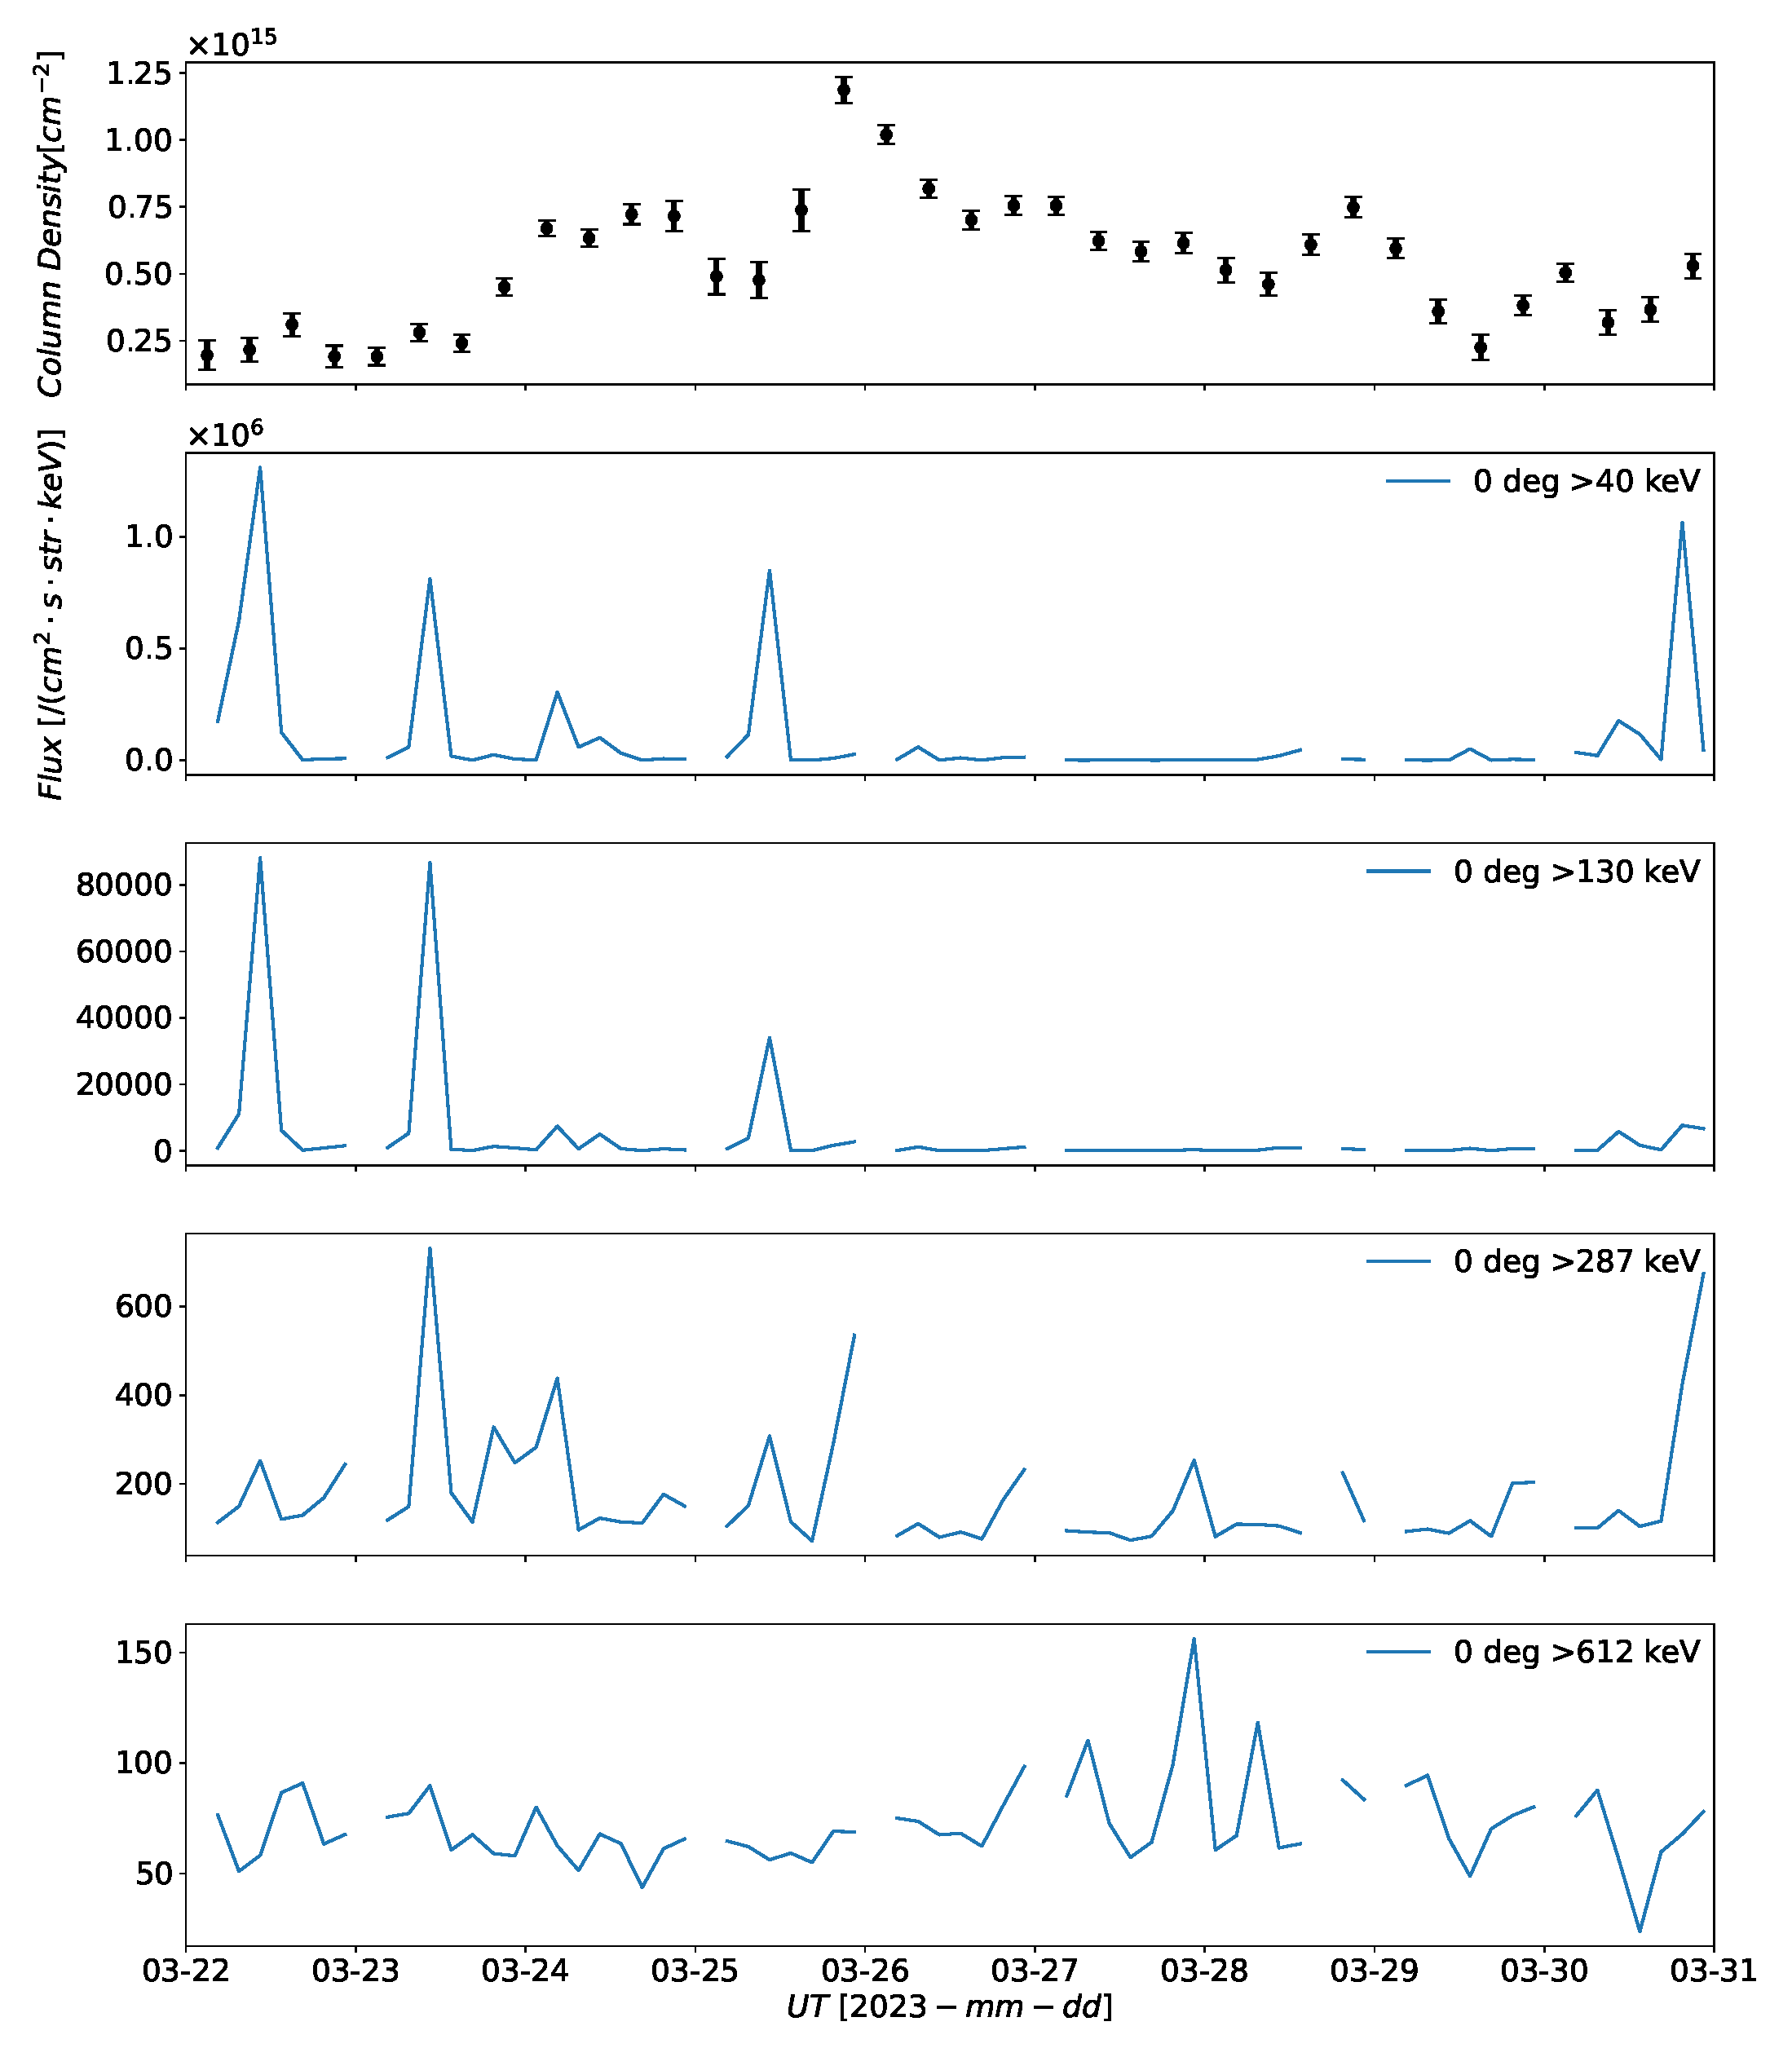
\includegraphics[width=\linewidth]{master_thesis_contents/master_thesis_fig/column_density_spectr6_poes0deg_syowa.pdf}
    \caption{昭和基地における柱密度(1段目。図~\ref{fig:column_density_spectr6_syowa}と同様)と電子フラックスデータ(2-5段目)との比較}
    \label{fig:poes_mmcd_syowa}
\end{figure} \par

トロムソと昭和基地どちらにおいても、すべての柱密度の増加がみられる期間に対応した電子フラックスの増加がみられた。
ただし、対応関係があることは確認できたが、電子フラックスの変動のタイムスケールと\ce{NO}の柱密度の変動のタイムスケールが一致しないということが分かった。
このことは、\ce{NO}の寿命が数日程度であることを考えると想定の範囲であると考えている。\par

まずトロムソのデータに関して詳しく見てみると、Dst指数の急激な減少と同時に、急激な\ce{NO}の柱密度の増加があった期間(2019年2月1日〜2019年2月4日)は、すべてのエネルギーレンジで電子フラックスの値が大きくなっており、とくに$>287\ \mathrm{keV}$や$>612\ \mathrm{keV}$などのエネルギーが大きい電子フラックスの値が上昇していることが確認できた。
また、Dst指数の減少が比較的小さく、\ce{NO}の柱密度の緩やかな増加があった期間(2019年1月23日〜2019年1月27日)については、どのエネルギーの範囲の電子フラックスの値も前者の現象と比べると小さいことが分かった。
これらは、\ref{ssec:comparison_dst}節で予想したようなEPPの影響によって\ce{NO}が増加したと考えられる。\par

次に昭和基地のデータについては、Dst指数の急激な減少と、\ce{NO}の柱密度の増加があった期間(2023年3月23日21時〜2023年3月24日3時)は、ほぼすべてのエネルギーレンジで電子フラックスの増加が確認された。
Dst指数の急激な減少が確認できなかったものの、\ce{NO}の柱密度の増加があった期間(2023年3月25日9時〜2023年3月25日21時)においても電子フラックスの増加が確認された。
さらに、柱密度の増加が確認できなかった期間(2023年3月22日)においても、比較的小さいエネルギーレンジ($>40\ \mathrm{keV}$, $>130\ \mathrm{keV}$)において電子フラックスの増加がみられた。
この3種類の異なる結果を合わせて考えると、比較的大きいエネルギーを持った電子が低い高度まで降り込むことで、\ce{NO}の生成効率を上げていると考えられる。
これは、理論的な予測(先行研究~\cite{turunen2009impact})とも矛盾しない(図~\ref{fig:turunen2009impact_fig3r})。
\begin{figure}[htbp]
    \centering
    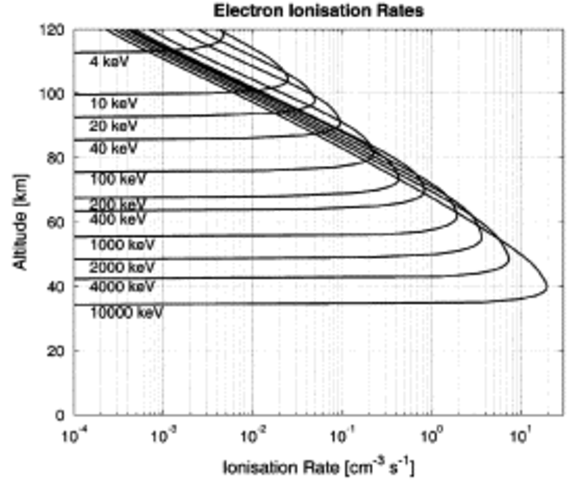
\includegraphics{master_thesis_contents/master_thesis_fig/turunen2009impact_fig3r.pdf}
    \caption{電子のエネルギーと降り込み高度の対応。この図より$>287\ \mathrm{keV}$の電子は高度70\ km付近まで降り込むことがわかる(~\cite{turunen2009impact}より引用)。}
    \label{fig:turunen2009impact_fig3r}
\end{figure} \par

これらのデータ比較から、\ce{NO}の増加に影響を与える高エネルギー降り込み電子の起源を探るため、磁気圏での物理状態を調べる必要があると考えた。
そのため、降り込む電子のソースとなる磁気圏と電離圏の様子を調べることができるOMNI Data Setを用いた比較を行った結果を次節に述べる。


\subsection{OMNI Data Setとの比較}
\label{ssec:comparison_omni}
降り込む粒子の物理量および磁気圏の物理状態と\ce{NO}増加量の関係を明らかにするため、降り込む電子のソースとなる磁気圏と電離圏の様子を調べることができるOMNI Data Set\footnote{\url{https://omniweb.gsfc.nasa.gov/form/omni_min.html}}を用いた比較を行った(OMNI Data Setの詳細は付録~\ref{app:omni})。
トロムソと昭和基地における比較結果をそれぞれ図~\ref{fig:omni_mmcd_tromsoe}、図~\ref{fig:omni_mmcd_syowa}に示す。
ここで、SYM/HはDst指数の1分値に相当するものであり、AE指数はサブストームに伴う電流の大きさを表すものである~\cite{wdc2009asysym,wdc2022onAEindex}。
昭和基地の解析した期間についてはAE指数は\today 時点で公開されていないため、昭和基地における柱密度との比較ではAE指数は用いていない。\par
% 仮綴じでは today = 2024-01-26となっている。
\begin{figure}[htbp]
    \centering
    \begin{minipage}{\linewidth}
        \centering
        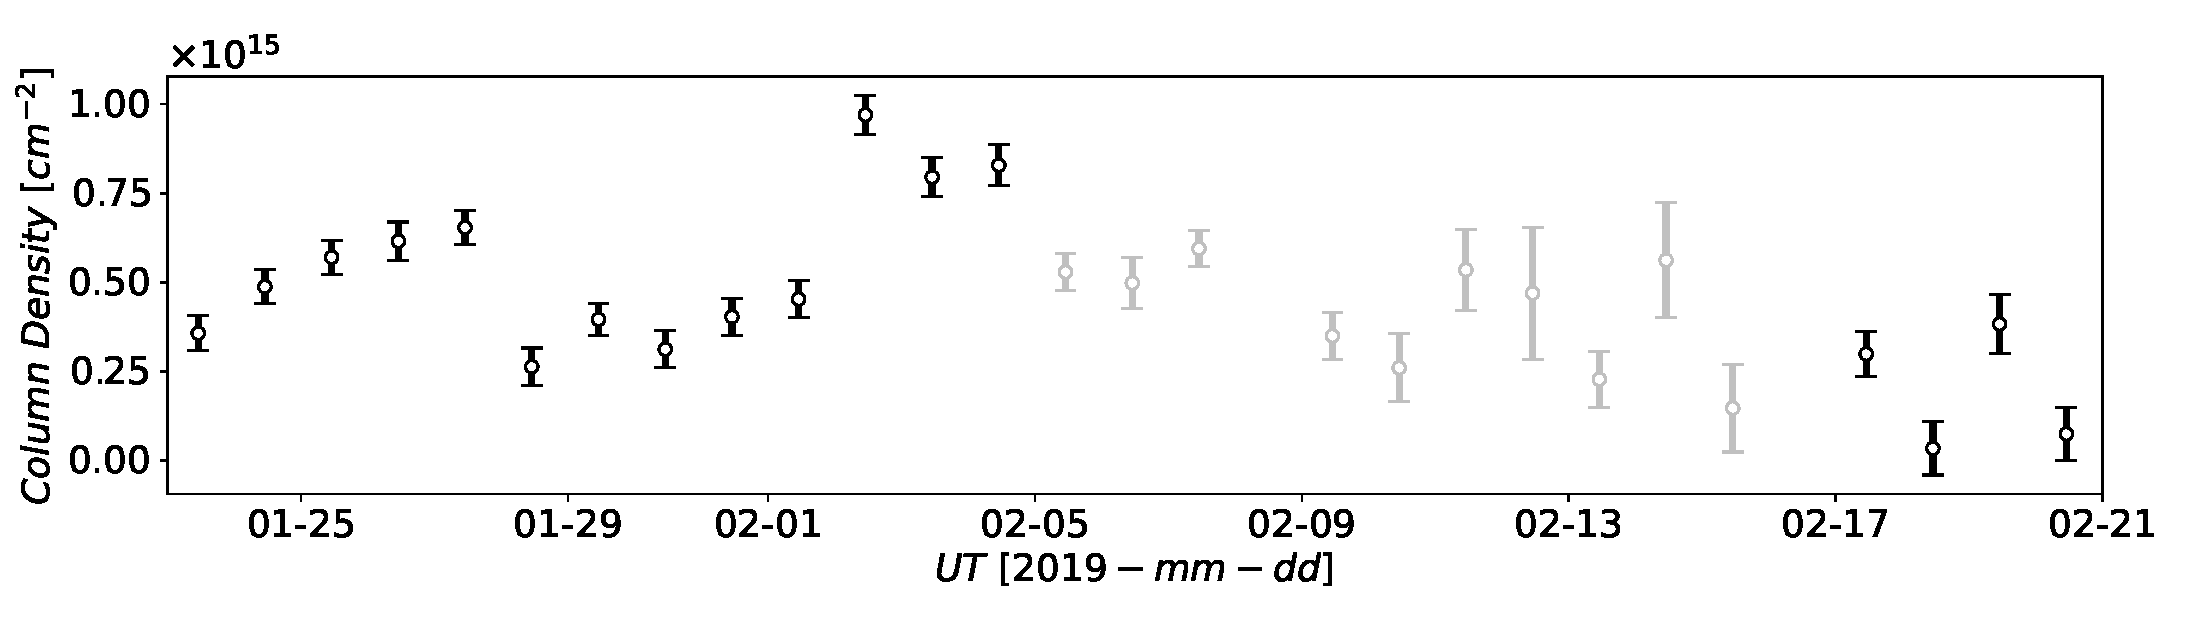
\includegraphics[width=\linewidth]{master_thesis_contents/master_thesis_fig/avg_ColumnDensity_tromsoe.pdf}
    \end{minipage}
    \begin{minipage}{\linewidth}
        \centering
        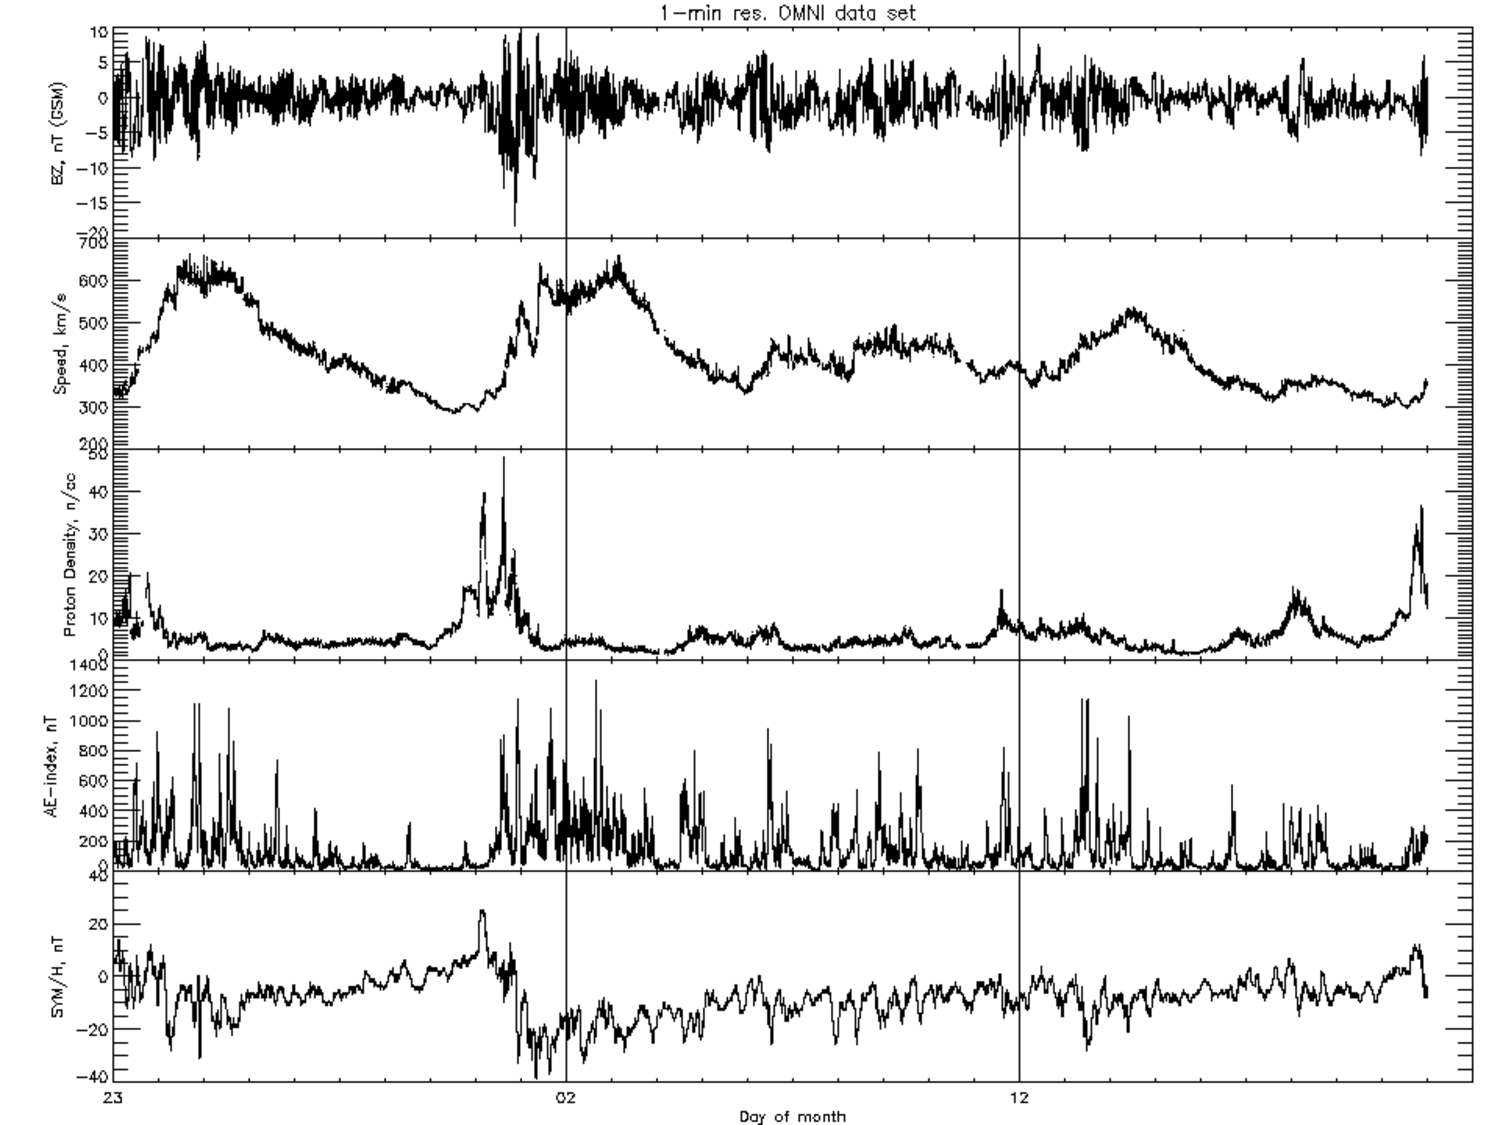
\includegraphics[width=\linewidth]{master_thesis_contents/master_thesis_fig/omni_tromsoe.pdf}
    \end{minipage}
    \caption{トロムソにおける柱密度(1段目。図~\ref{fig:avg_ColumnDensity_tromsoe}と同様)とOMNI Data Set(2段目:地球磁場の南北成分、3段目:太陽風の速さ、4段目:プロトン密度、5段目:AE指数、6段目:SYM/H)との比較}
    \label{fig:omni_mmcd_tromsoe}
\end{figure}

まずトロムソにおいては、柱密度の増加が確認された2つの期間(2019年1月23日〜2019年1月27日と2019年2月1日〜2019年2月4日)どちらにおいても、地球磁場の南北成分のゆらぎが確認できた。
また、太陽風の速さも大きくなっており、AE指数も何度も激しく値が上昇している。
以上より、SYM/H(もしくは図~\ref{fig:dst_mmcd_tromsoe}のDst指数)の値をみると磁気嵐としての規模に違いはあるが、対象の期間では高速太陽風が吹いており、サブストームが活発にあったことが考えられる。
このことより、高速太陽風が到達した際に磁気圏の活動が活発となり、電子が降り込むことで\ce{NO}の変動に影響を与えたと考えられる。
また、2019年2月1日〜2019年2月4日の期間においては、プロトンの密度も上昇していることが確認された。\par
\begin{figure}[htbp]
    \centering
    \begin{minipage}{\linewidth}
        \centering
        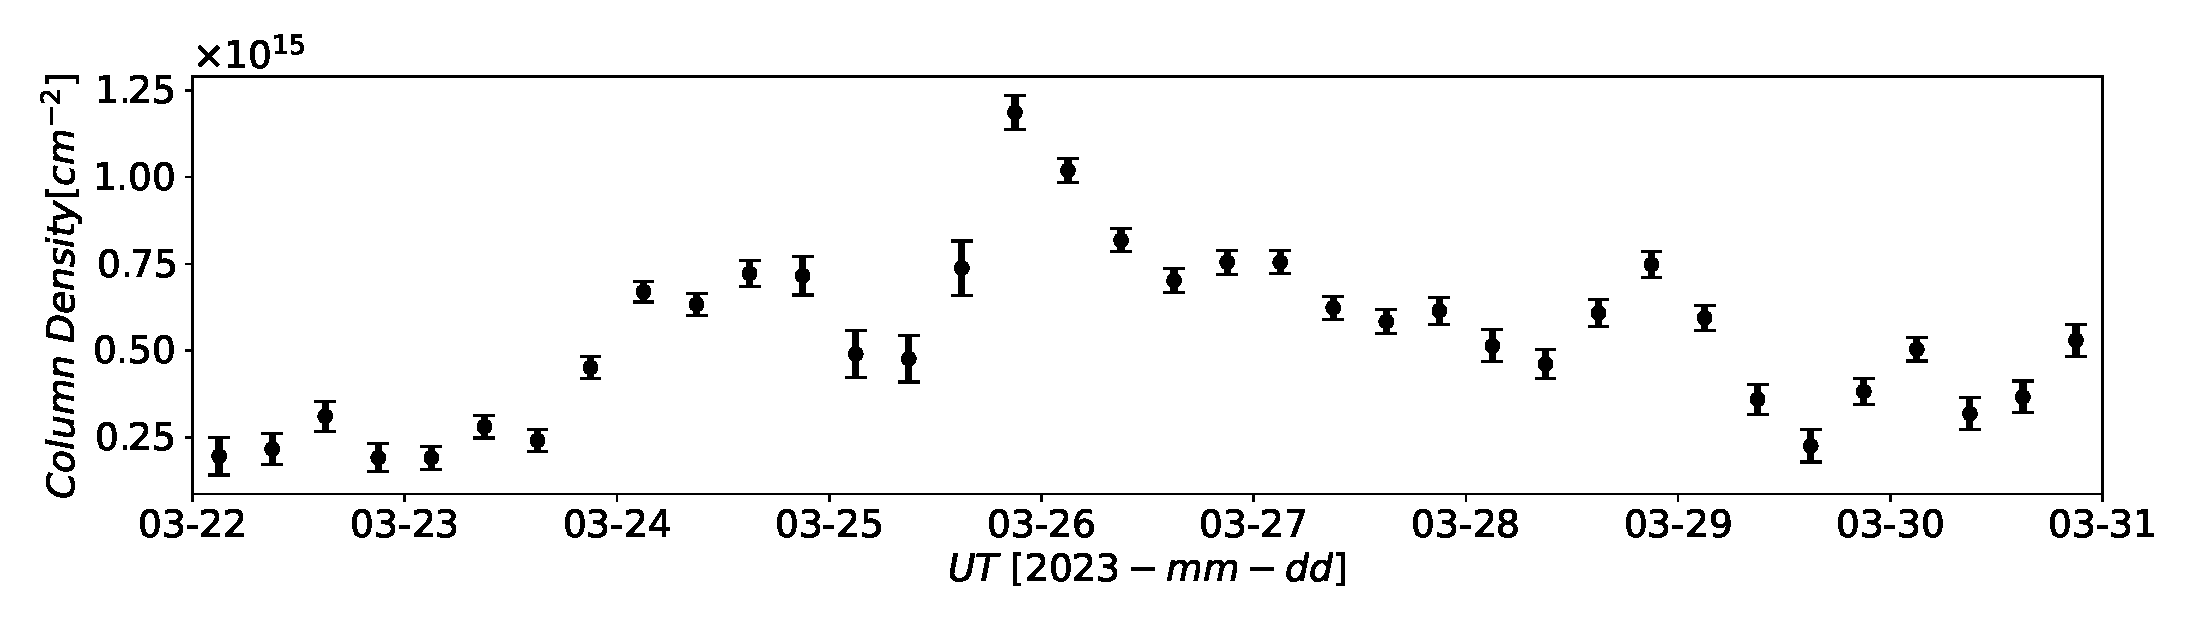
\includegraphics[width=\linewidth]{master_thesis_contents/master_thesis_fig/column_density_spectr6_syowa.pdf}
    \end{minipage}
    \begin{minipage}{0.96\linewidth}
        \centering
        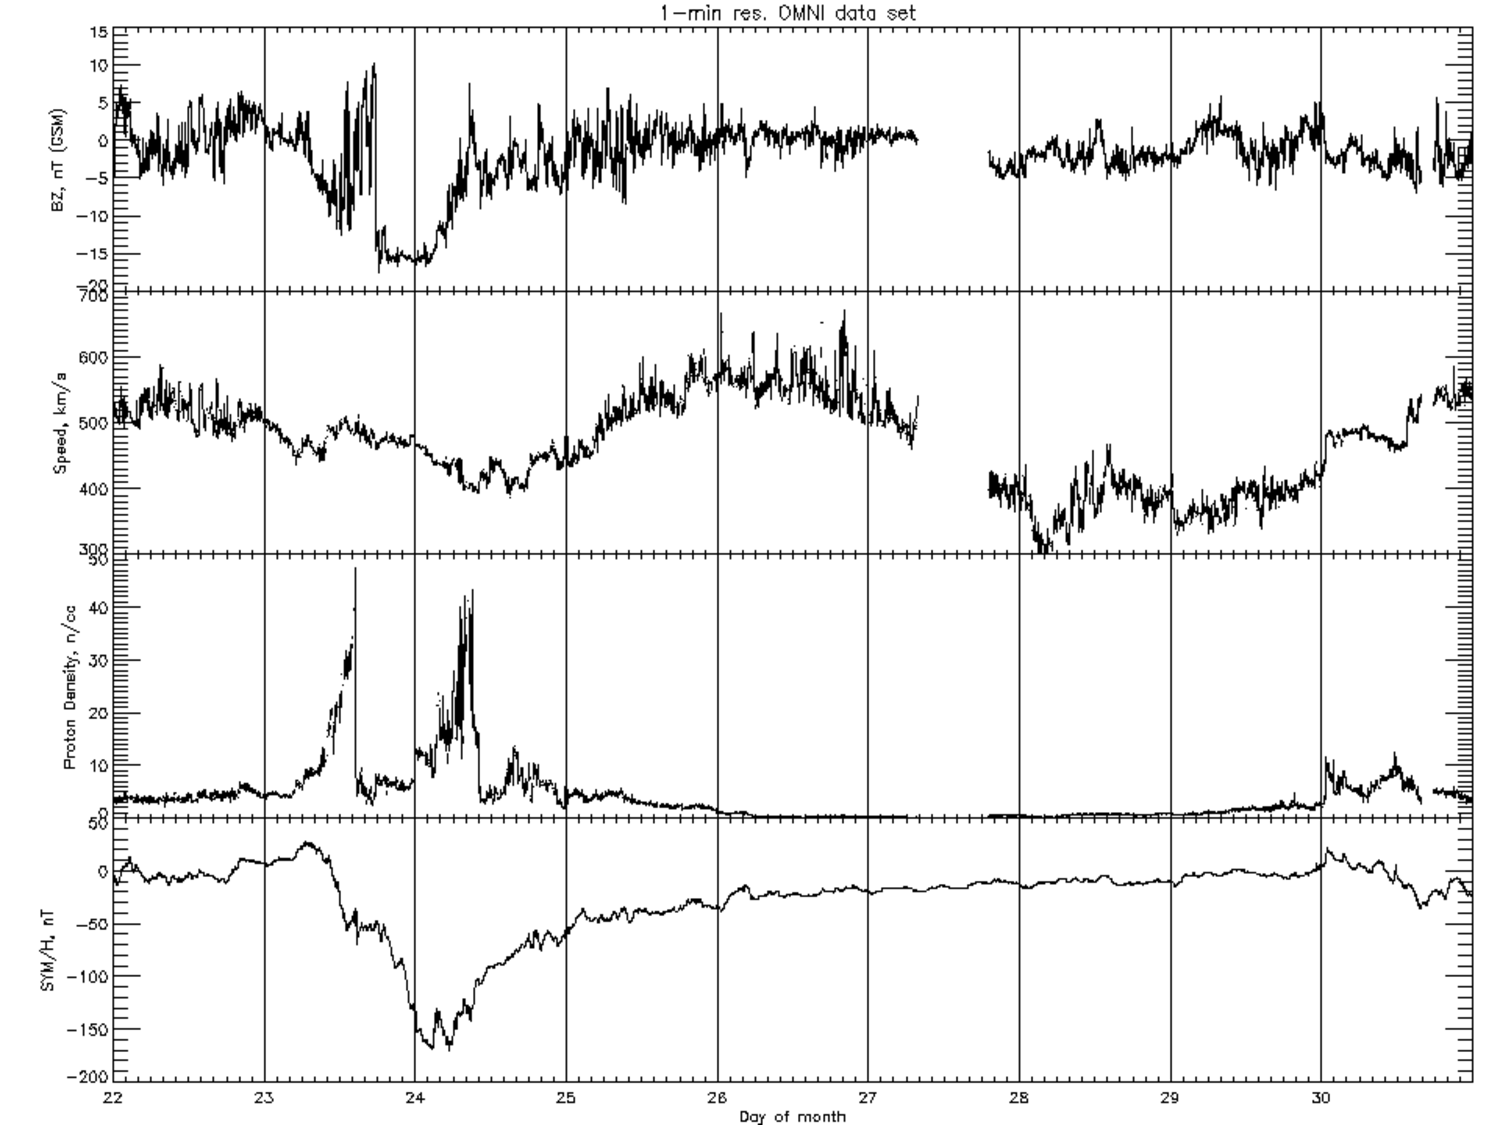
\includegraphics[width=\linewidth]{master_thesis_contents/master_thesis_fig/omni_syowa.pdf}
    \end{minipage}
    \caption{昭和基地における柱密度(1段目。図~\ref{fig:avg_ColumnDensity_tromsoe}と同様)とOMNI Data Set(2段目:地球磁場の南北成分、3段目:太陽風の速さ、4段目:プロトン密度、5段目:SYM/H)との比較}
    \label{fig:omni_mmcd_syowa}
\end{figure}

次に昭和基地においては、磁気嵐の発生と対応して柱密度が増加した2023年3月23日〜2023年3月24日において地球磁場が南方向を向いており、プロトンの密度も上昇していることが確認された。
しかし、高速太陽風は確認できなかった。
もう1つ柱密度の増加が確認できた2023年3月25日においては、SYM/H(もしくは図~\ref{fig:dst_mmcd_syowa}のDst指数)の値をみると磁気嵐は回復相にあたるが、高速太陽風があることが確認できた。
このことより、磁気圏から回復する期間であっても高速太陽風が到達していると電子の降り込みがあり、\ce{NO}の増加に影響を与えると考えられる。
また、この時期の磁場の振動の中心はわずかに(数nT程度)南向きの状態において高速太陽風が到達しているが、同様な条件で電子フラックスの値が増加することが先行研究~\cite{miyoshi2013high}にて示されている。
